\documentclass[12pt,conference]{IEEEtran}

% Preset Packages
\usepackage{cite}
\usepackage[hyphens]{url}
\usepackage{hyperref}
\usepackage{amsmath,amssymb,amsfonts}
\usepackage{algorithmic}
\usepackage{fancybox, graphicx}
\usepackage{textcomp}
\usepackage{xcolor}
\usepackage{csquotes} % Used to display quotes
\def\BibTeX{{\rm B\kern-.05em{\sc i\kern-.025em b}\kern-.08em
    T\kern-.1667em\lower.7ex\hbox{E}\kern-.125emX}}

% Set the path to keep diagram images
\graphicspath{ {Images/} }

% Create a "todo" style (just red text)
\newcommand\todo[1]{\textcolor{red}{#1}}

% =============================================================================
% =  BEGINNING OF THE DOCUMENT
% =============================================================================
\begin{document}

% Include Page Numbers
\pagenumbering{arabic}
\pagestyle{plain}

% Create the title
\title{Structural Quality \& Software Evolution: \newline First Draft}

%% =============================================================================
% =  Author Information
% =============================================================================
\author{
\IEEEauthorblockN{Alison Major}
\IEEEauthorblockA{\textit{Department of Computer and Mathematical Sciences} \\
\textit{Lewis University}\\
Romeoville, Illinois, USA \\
AlisonMMajor@lewisu.edu}
}

% =============================================================================
% =  Paper Title
% =============================================================================
\maketitle
% \tableofcontents

% =============================================================================
% =  Paper Abstract
% =============================================================================
\begin{abstract}

% State the problem.
Some software engineering projects fail to evolve, which leads to them becoming obsolete.
% Say why this problem is interesting.
This topic is interesting and important to developers because software that fails to evolve will fail to generate user engagement, which leads to loss of revenue.
% Say what my solution achieves.
\todo{Say what my solution achieves.}
% Say what follows from my solution.
\todo{Say what follows from my solution.}

\end{abstract}

% =============================================================================
% =  Introduction (1 page)
% =============================================================================
\section{Introduction}

When building systems as software engineers, we have several areas of concern. How much will it cost? How long will it take to deliver? What will the quality be? Often, the cost and time-to-market are the two concerns given the highest priority in a project. However, the quality must be considered to preserve the system's longevity.

One way to understand the quality around a system is to discuss its ``maintainability,'' that is, the ease of receiving new features or resolving bugs. For example, if a system is tightly coupled, it may be that adjusting one area to add a new feature requires touching several other parts of the system.

To give some simple examples for tightly and loosely coupled systems, let us consider your eyes. If you are a near-sighted individual, a loosely coupled solution to improve your vision is to get glasses or contacts. You can change out the glasses for different types and styles while providing a solution to your problem (poor vision). However, you cannot simply change your eyes; these are tightly coupled to your body and would be difficult to remove and swap for another set of eyes without considerable work to separate and reattach them to the correct systems. By having a loosely coupled system (wearing glasses), we allow for easy feature changes (turn those glasses into sunglasses! pick a new style!) and easy bug fixes (adjust the prescription).

Like how it may be easier to change how we look and how well we can see by using prescriptive eyewear, creating a structured software system will impact how the software can evolve with new features. If a system is difficult to evolve, users will lose favor as it cannot offer the newest features that competitors may offer.

\todo{State your contributions. Do not leave the reader to guess what my contributions are. Should be provable (refutable). Contributions will be things we have proven or worked out in the following sections. Can link to those sections as we describe those contributions.}

\todo{CLAIM: We can use maintainability scores to see how structure impacts evolution} (Section \ref{sectionMaintainabilityScores}).

\todo{CLAIM: Following shared standards improves maintainability} (Section \ref{sectionSharedStandards}).

\todo{CLAIM: Documentation can improve maintainability} (Section \ref{sectionDocumentation}).

% =============================================================================
% =  The Problem (1 page)
% =============================================================================

\section{The Problem \todo{TODO: Rename Section}}
\todo{TODO: the problem - 1 page}

% --- The problem is that some projects fail to evolve ------------------------

When developing a new system, a new software idea, getting the project off the ground and in front of users is one thing. However, it is another thing to keep that project alive with a thriving community of engaged users.

The systems we create could be customer-facing web applications, games, or internal applications used within a business to carry out tasks. Regardless of the type of system, without evolving with the user's needs, the product will no longer provide usefulness. However, even in the business world with internal systems, needs change, and how a system must be used needs to have enough flexibility for tasks to continue to be completed.

Let's consider what software evolution is, from this simple definition on Wikipedia \cite{wiki:software-evolution}:

\begin{displayquote}
Software evolution is the continual development of a piece of software after its initial release to address changing stakeholder and/or market requirements.
\end{displayquote}

% --- Why does it matter if a project does not evolve? ------------------------

When a system cannot evolve, the users mainly feel the impact. However, this impact will eventually get back to those who created and continue to support the system. With users that are either unsatisfied or unable to use the system any longer, the engagement levels will drop, and so will the users. This will ultimately result in a loss of income, as the system can no longer deliver to the needs of its audience.

Because organizations invest large amounts of money in the software systems that they create, they are dependent on the continued success of the software. Software evolution will allow the system to adapt to new or changing business requirements, fix bugs and defects, and also integrate with other systems that have changed and evolved that may share the same software environment.

As a system is used, inevitably users will stumble into situations that even the best quality assurance testers will miss. When defects are found, they will require fixing. 

To keep a system up-to-date, we must add new features. There may be needs to improve performance or reliability of a system, especially if the user-base expands.

Security can also impact the needs for a system to be maintained. New ways to infiltrate a system can be uncovered, so it is important to stay on top of newest versions of dependencies and technologies in order to avoid potential breaches of data and experience.

% --- How do we ensure a project will be able to evolve? ----------------------

Because the maintainability of a system can ultimately influence the ability to generate revenue, we must find ways to ensure that a project will evolve. One of these ways could be to ensure that a project continues to be considered ``maintainable'' throughout its lifetime. This characteristic of a system will ensure that bugs can be fixed quickly, but new features should be easy to add as the users' needs evolve.

If a system is large, it may involve a number of steps in order to get changes through. For example, a process like that in ``Fig.~\ref{figLargeSystemMaintenance}'' shows 7 indivudal steps just to get to a new feature release. Any amount of complexity can make this processes even more cumbersome.

\begin{figure}[ht]
    \centerline{
        \includegraphics[width=\columnwidth]{Maintenance_LargeSystem}
    }
    \caption{Large systems take a number of steps to add new features.}
    \label{figLargeSystemMaintenance}
\end{figure}

\todo{examples? anything about other evolution processes? better diagrams?}
\todo{See example diagrams by searching for ``software evolution'' on google}

\begin{figure}[ht]
    \centerline{
        \includegraphics[width=\columnwidth]{AddingNewFeatures}
    }
    \caption{New features are part of the evolution process.}
    \label{figAddingNewFeatures}
\end{figure}

% =============================================================================
% =  My Idea (2 pages)
% =============================================================================

\section{The Impact of Structural Quality}
\todo{TODO: my idea - 2 pages}


% --- Understand Software Maintenance -----------------------------------------
\subsection{Understand Software Maintenance}

The structural quality of a software system will impact the software evolution. If the project has poor structural quality, its ability to evolve will be minimized and the software system will eventually ``die-off'' so to speak.

There is much planning involved in all software creation projects in what the product will be, will do, who it is for, and so on. One of the things that should also be on the planning list is for long-term maintenance and growth. That is, how do we build a thing that will be easier to add features to down the road?

Let us define maintainability in the context of software. For example, a system would be considered easy to maintain if it is easy to debug and adds new features.

It may be easier to understand what characteristics define a system with poor maintainability. These types of systems will have poor code quality, leading to defects. For example, there could be undetected vulnerabilities or have been ignored. However, it may be that the system is overly complex. In addition to the complexity, it could be hard to read due to poor naming or dead (unused) code throughout the source code.

A project is known to have good maintainability when there is an enforced set of clean and consistent standards for the code. This often involves having human-readable names for functions, methods, and variables. Any complex code is minimized, and methods are small and focus on a single thing. Parts of the system are decoupled and organized, making it easy to work on different parts with low impact on unrelated parts. For example, the code is DRY (there is limited redundancy), unused code has been removed, and there is a level of documentation that supports an easy understanding of the system.

Why should we care about whether the code is maintainable? It is assumed that a large amount of the cost over the lifetime of a project is attributed to maintainability. Fred Brooks, in his book ``The Mythical Man-Month'' even claimed that over 90\% of the costs for a typical software system come up in the maintenance phase \cite{brooks:mythical}. Once the bulk of the system is off the ground and live worldwide, how well the team can improve the system with new features and by fixing bugs can be impacted by its maintainability. Any successful piece of software will inevitably need to be maintained.

% --- Understand Software Evolution -------------------------------------------
\subsection{Understand Software Evolution}

There is a distinction to be made between \textbf{software maintenance} and \textbf{software evolution}. Software maintenance is what we'll refer to as bug resolution and for minor enhancements. For example, when we must fix a broken route in the application, or provide subtle improvement on the user experience, we can consider this normal maintenance. However, when we look at upgrades to the system, adaptations to the changing and growing needs of the user, or migrating the system to a new technology, we can refer to this as evolution of the software.

Evolution of software can be a result of new laws that have come into being. As technology itself changes, governing bodies must continually revisit policies on data collection and information sharing. This may lead to adaptations that result from the new laws, or even adaptations to take advantage of new technlogies.

It is also fair to say that systems will change because we can never fully determine the needs of a user at the start of a project. In fact, it would be safe to say that the needs of the user will change over time themselves. This leads to a never-ending project that will always need some form of enhancements.

Meir "Manny" Lehman and László "Les" Bélády contributed to a list of laws involving software evolution known as Lehman's Laws that describe a balance between forces that drive new developments while also slowing progress. These laws specifically apply to programs that were written to perform some real-world activity, where its behavior is linked to the environment in which it runs; additionally, this program category assumes that the program needs to adapt to varying requirements and circumstances in that environment. Eight laws were created and are summarized below.
\cite{wiki:lehmans-laws}

\begin{enumerate}
    % "Continuing Change" — an E-type system must be continually adapted or it becomes progressively less satisfactory.
    \item \textbf{Continuing Change} \textit{(1974)}
    
    % "Increasing Complexity" — as an E-type system evolves, its complexity increases unless work is done to maintain or reduce it.
    \item \textbf{Increasing Complexity} \textit{(1974)}

    % "Self Regulation" — E-type system evolution processes are self-regulating with the distribution of product and process measures close to normal.
    \item \textbf{Self Regulation} \textit{(1974)}

    % "Conservation of Organisational Stability (invariant work rate)" — the average effective global activity rate in an evolving E-type system is invariant over the product's lifetime.
    \item \textbf{Conservation of Organisational Stability} \textit{(1978)}

    % "Conservation of Familiarity" — as an E-type system evolves, all associated with it, developers, sales personnel and users, for example, must maintain mastery of its content and behaviour to achieve satisfactory evolution. Excessive growth diminishes that mastery. Hence the average incremental growth remains invariant as the system evolves.
    \item \textbf{Conservation of Familiarity} \textit{(1978)}

    % "Continuing Growth" — the functional content of an E-type system must be continually increased to maintain user satisfaction over its lifetime.
    \item \textbf{Continuing Growth} \textit{(1991)}

    % "Declining Quality" — the quality of an E-type system will appear to be declining unless it is rigorously maintained and adapted to operational environment changes.
    \item \textbf{Declining Quality} \textit{(1996)}

    % "Feedback System" (first stated 1974, formalised as law 1996) — E-type evolution processes constitute multi-level, multi-loop, multi-agent feedback systems and must be treated as such to achieve significant improvement over any reasonable base.
    \item \textbf{Feedback System} \textit{(1996)}
\end{enumerate}

The first law, ``Continuing Change,'' tells us that if a system does not continue to adapt, it will become progressively less satisfactory. The second, ``Increasing Complexity,'' explains that as a system evolves, unless work is done to maintain or reduce complexity, the complexity will increase. This can be due the added volume of the code from new features, or even as a result of an increasing number of developers that have edited the code. Unless this phenomenon of increased complexity is actively addressed during changes, it can impact the maintainability (and the ability of a project to continue evolving) in the future.

Lehman's fifth law, ``Conservation of Familiarity,'' explains how the average incremental growth does not change over time as a system evolves. The people interacting with the system, such as the developers, business personel, or users, must still be able to continue to use and work within the system at the same ``level of mastery.'' If the system grows and changes excessively, the mastery of the system will drop, slowing down the next set of changes. This could be because the source code or architecture has become more complex (impacting the developers' ability to adapt and enhance the system) or because the user features have changed in such a way that the system audience needs time to master the new interfaces or new tools. Because of this natural ``slow-down'' for excessive change occurs, the average incremental growth will remain steady. We can see a simplified visual in ``Fig.~\ref{figConservationOfFamiliarity}'' showing that when the number of changes spikes (that is to say, when there is excessive growth in a system), it will be followed by an iteration of fewer changes, leading to a nearly consistent average of incremental growth (the thick, horizontal line) over time.

\begin{figure}[ht]
    \centerline{
        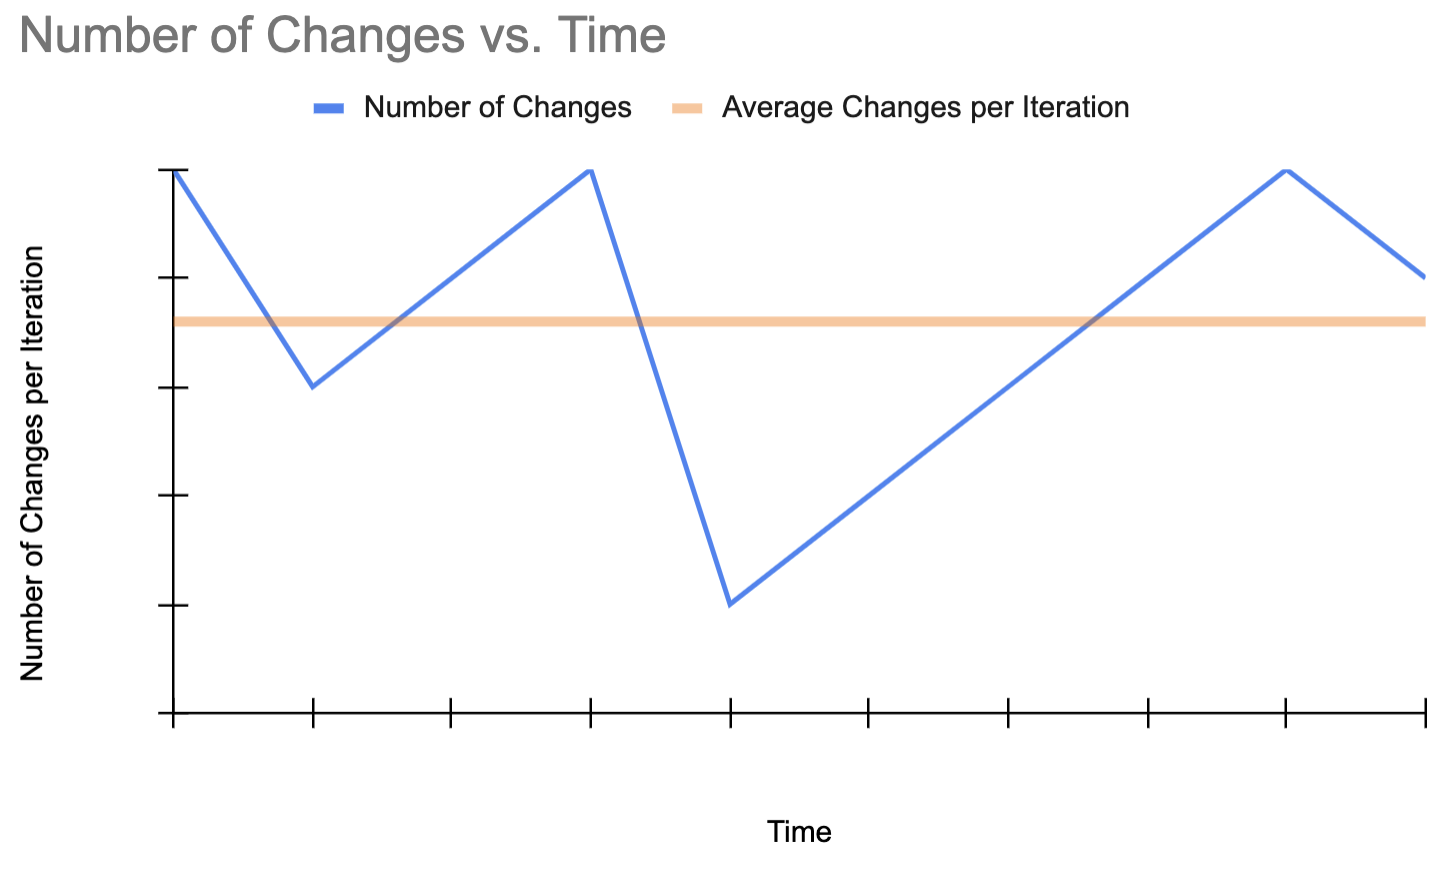
\includegraphics[width=\columnwidth]{Changes-vs-Time}
    }
    \caption{A simplified visual of Lehman's fifth law, ``Conservation of Familiarity.''}
    \label{figConservationOfFamiliarity}
\end{figure}

In Lehman's sixth law, ``Continuing Growth,'' we see that the system user's satisfaction will not be maintained without continually increasing the functional content. Along a similar idea, the law pertaining to ``Declining Quality'' states that if the operational environment for the system does not change, the quality of the system will appear to decline. We must continue adapting for even the appearance of maintained quality of a system.

With all of these characteristics surrounding the evolution of software, we have the benefit of the Internet that has positively improved the experience. Two common resources currently available to developers have impacted software evolution \cite{wiki:software-evolution}:

\begin{enumerate}
    \item The rapid growth of World Wide Web and Internet Resources make it easier for users and engineers to find related information.
    \item Open source development where anybody could download the source codes and hence modify it has enabled fast and parallel evolution (through forks).
\end{enumerate}

These two suggestions are evident if you are a developer. It is quite possible that you regularly use resources like StackOverflow to find solutions to problems, as well as using open source tools that you and your team can contribute to or adjust to your specific needs.

\subsection{Measuring Maintainability}

Despite the nuanced differences between \textit{maintainability} and \textit{evolution}, the two characteristics run parallel to each other. If a system is easy to maintain, it follows that it will also be easier to evolve. If we can measure our system's maintainability, we can also determine if our system is in a good position to continue evolving to meet our future needs.

Several tools attempt to provide some value around these ideas. In this paper, we will focus on the metrics that Pylint provides, specifically looking into the Refactor score of Pylint.

We will look at many open-source Python systems using Pylint and attempt to correlate the data from the Pylint scores to the level of ease in adding new features to the system. This will determine if a system is more maintainable when it has better Pylint scores. To do this, we will measure the locality of the changes by the number of files that are edited in a commit. We will also focus on commits that represent new features, not on commits that are bug fixes.

\todo{any examples for this section?}

% =============================================================================
% =  The Details, defending my idea (5 pages)
% =============================================================================

\section{The Details \todo{TODO: Rename Section}}
\todo{TODO: the details - 5 pages}

% --- How does my idea solve the problem? -------------------------------------
% --- THE PROBLEM: Some projects fail to evolve, resulting in loss if income.
% --- MY IDEA: Software evolution is impacted by structural quality.
% -----------------------------------------------------------------------------

Now that we have established that we have a problem with projects that fail to evolve, which can result in a loss of revenue, we need to understand how we can ensure that our systems may evolve. For this, we will look to understand how the evolution of software is impacted by the system's structural quality.

% -----------------------------------------------------------------------------
% -  (A) We can use maintainability scores to see how structure impacts evolution.
% -----------------------------------------------------------------------------
\subsection{Maintainability Scores} \label{sectionMaintainabilityScores}

% --- Claim A: Review each claim from the introduction

First, let us consider our original understanding about software maintainability. While this particular definition is focused primarily on bug fixes and minor enhancements, projects that are maintainable should also have an ease in their ability to evolve over time. Therefore, we can study the impact maintainability (that is, structural quality) has on software evolution by reviewing the scores provided by automated code review tools.

In this study, we will be using Pylint and will be focused on the values of the Refactor score in regards to a set of open-source Python systems. To understand the scores we will be working with, we must understand what Pylint itself is doing. 

\todo{Through the documentation of Pylint, we can understand how to use it and the scores it will provide \cite{pylint:main}.}

\todo{We can also review the documentation to know how the Pylint Score is calculated, as well as the various features that the Refactor Score takes into account \cite{pylint:score}.}

Finally, in respect to Python, it is also essential to understand PEP 8, as this is the default set of standards that Pylint uses to judge Python code \cite{pylint:pep8}. This standard can be used to make code more readable, which in turn, may contribute to the code being more maintainable.

% --- Claim A: Identify the evidence (analysis and comparison, theorems, measurements, case studies)

The authors of ``Measurement and refactoring for package structure based on complex network'' recently reviewed a similar idea with the focus on cohesion and coupling over time for a project \cite{zhou:2020}. In a software system, we desire low coupling (allows for changes to one area to remain independent of changes to another area of a system) and high cohesion (indicates reduced complexity in modules, which improves maintainability). 

\todo{TODO: read and understand their findings and see how it compares to the data that we collect and understand.}

Another variable that may impact the maintainability of code is readability. For example, in the article ``How does code readability change during software evolution?'' the authors have addressed this concern and found that most source codes were readable within the sample they reviewed. Additionally, a minority of commits changed the readability \cite{piantadosi:2020}. This variable in the maintainability of a software system can influence how easy or difficult it is to make a change. 

\todo{TODO: compare guidelines from \cite{piantadosi:2020}; do best scoring projects follow these ideas?}

Another paper, ``Standardized code quality benchmarking for improving software maintainability,'' provides additional insights into how the code's maintainability is impacted by the technical quality of source code \cite{baggen:2012}. Within their paper, the authors seek to show four key points: (1) how easy it is to determine where and how the change is made, (2) how easy it is to implement the change, (3) how easy it is to avoid unexpected effects, and (4) how easy it is to validate the changes. 

\todo{TODO: compare \cite{baggen:2012} to our data}

% -----------------------------------------------------------------------------
% -  (B) Following shared standards improves maintainability.
% -----------------------------------------------------------------------------
\subsection{Shared Standards} \label{sectionSharedStandards}

% --- Claim B: Review each claim from the introduction

\todo{Reviewing the ``Systems and software engineering — Systems and software Quality Requirements and Evaluation (SQuaRE) — System and software quality models'' maintained by ISO may also provide interesting insights \cite{iso/iec:25010:2011}. Does the Pylint checker follow the quality models outlined here? Are there benefits or drawbacks to the models that the ISO/IEC:25010:2011 suggests? These could influence more thoughts on interpreting final data results.}

% --- Claim B: Identify the evidence (analysis and comparison, theorems, measurements, case studies)

\todo{TODO: Claim B - identify evidence (analysis and comparison, theorems, measurements, case studies).}

% -----------------------------------------------------------------------------
% -  (C) Documentation can improve maintainability.
% -----------------------------------------------------------------------------
\subsection{Documentation} \label{sectionDocumentation}

% --- Claim C: Review each claim from the introduction

We can see that the Refactor score in projects correlates to the evolution of the system \todo{(TODO: Confirm this)}. This may indicate that the code and system are readable in themselves, in addition to being loosely coupled and highly cohesive. Out of curiosity, we can also review the level of documentation in several of the most maintainable projects, as well as several of the least maintainable projects. It would be useful to understand if there are any similarities in how a system is documented that could contribute to improved software evolution of a system.

\todo{TODO: what kind of docuemntation do the ``good'' projects have?}

\todo{TODO: what kind of docuemntation do the ``bad'' projects have?}

% --- Claim C: Identify the evidence (analysis and comparison, theorems, measurements, case studies)

The course textbook, ``Software Architecture in Practice,'' chapter 18 provides some insight in documentation around architecture \cite{book:software-architecture-in-practice}. 

\todo{TODO: Do these projects have adequate documentation?}

\todo{TODO: Does the level of documentation correlate to the ability to maintain a decent score?}

% =============================================================================
% =  Related Works (1 to 2 pages)
% =============================================================================

\section{Related Work}
\todo{TODO: related work - 1 to 2 pages - give credit to those who have come before, 1-2 pages}

The work done by Dr. Omari and Dr. Martinez involves collecting a sub-set of Python projects that we can use for further research. The bulk of the effort they have provided is determining which classifiers to use to pare down the public set of Python systems into a good collection for further analysis \cite{omari:2018}. The work that they ahve provided was used to select appropriate Python systems for review by collecting meta-data on these code systems.

\todo{TODO: elaborate more on Omari and Martinez work and influence}

A study conducted by Baishakhi Ray, Daryl Posnett, Premkumar Devanbu, and Vladimir Filkov begins by programmatically collecting a sample set of projects in GitHub that vary in languages. Then the group of projects was appropriately culled, resulting in a final set used for the review. The results were then studied for the impact different programming languages may have had on the code quality \cite{baishakhi:2017}. 

\todo{TODO: can these ideas provide direction and assumptions in our research?}

% =============================================================================
% =  Conclusions and Further Work (0.5 page)
% =============================================================================

\section{Conclusions \& Further Work}
\todo{TODO: conclusion - half page}

By collecting data and drawing our conclusions from it, with help from the insights from the studies done before ours, we may better understand metrics that can be useful in regards to maintainability. Good projects will inevitably continue to grow and evolve. Understanding methods to keep code refactor on a level that makes code easy to change. We may also find that projects with worsening scores slow down with updates and have reduced engagement.

\todo{TODO: did bad scoring projects die off?}

Projects that may be open source or have many contributors are especially vulnerable to maintainability degrading over the evolution of a project. Having a reliable metric can be very useful in programmatically avoiding code smells and keeping code in a state that is easy to manage through simple metric checks in deployment pipelines.

\todo{TODO: elaborate.}

Understanding the impact of structural quality on the evolution of a project can provide compelling perspectives.

% =============================================================================
% =  Bibliography and Sources
% =============================================================================
\newpage
\bibliographystyle{unsrt}
\bibliography{bibliography}

% =============================================================================
% =  END OF THE DOCUMENT
% =============================================================================
\end{document}
